\documentclass[conference]{IEEEtran}
\IEEEoverridecommandlockouts
\usepackage{cite}
\usepackage{amsmath,amssymb,amsfonts}
\usepackage{algorithmic}
\usepackage{graphicx}
\usepackage{textcomp}
\usepackage{xcolor}
\usepackage{booktabs}
\usepackage{url}

\def\BibTeX{{\rm B\kern-.05em{\sc i\kern-.025em b}\kern-.08em
    T\kern-.1667em\lower.7ex\hbox{E}\kern-.125emX}}

\begin{document}

\title{Hybrid Neuro-Symbolic Fake News Detection System\\
\thanks{Identify applicable sponsor/funding agency here. If none, delete this.}
}

\author{
\IEEEauthorblockN{C Naga Rohith}
\IEEEauthorblockA{\textit{Department of Electronics and Communication Engineering} \\
\textit{Amrita Vishwa Vidyapeetham}\\
Kerala, India \\
nagarohithchintala4@gmail.com}
\and
\IEEEauthorblockN{C Hari Dhanush}
\IEEEauthorblockA{\textit{Department of Electronics and Communication Engineering} \\
\textit{Amrita Vishwa Vidyapeetham}\\
Kerala, India \\
bobbydhanush24@gmail.com}
\and
\IEEEauthorblockN{PJSR Karthik}
\IEEEauthorblockA{\textit{Department of Electronics and Communication Engineering} \\
\textit{Amrita Vishwa Vidyapeetham}\\
Kerala, India \\
karthikponnaganti13@gmail.com}
}

\maketitle

\begin{abstract}
Fake news propagation through social media and online platforms has become a major societal challenge. Traditional machine learning approaches provide reasonable classification accuracy but often fail to explain the reasoning behind predictions. This project proposes a Hybrid Neuro-Symbolic Fake News Detection System that combines Machine Learning, Deep Learning, semantic verification, forensic analysis, and explainable reasoning for misinformation detection. The system integrates TF-IDF based Logistic Regression, BERT contextual analysis, semantic similarity verification, temporal consistency analysis, spatial consistency verification, and source validation using APIs. Unlike conventional black-box systems, the proposed framework generates rationale along with predictions to improve transparency and trustworthiness. Experimental results demonstrate that the hybrid system achieves approximately 89\% accuracy while improving interpretability and robustness against misleading content.
\end{abstract}

\begin{IEEEkeywords}
Fake News Detection, BERT, NLP, Neuro-Symbolic AI, Explainable AI, Semantic Similarity
\end{IEEEkeywords}

\section{Introduction}
The rapid growth of digital media and social networking platforms has significantly increased the spread of fake news and misinformation. False information can influence public opinion, create social panic, manipulate elections, and affect public trust. Since millions of online posts are generated every day, manual verification becomes difficult and time-consuming. Therefore, automated fake news detection systems have become an important area of research.

Conventional fake news detection methods mainly rely on machine learning algorithms trained on textual features. Although these techniques provide good classification accuracy, they often behave like black-box systems and fail to provide interpretable explanations for predictions. Recent advancements in transformer-based Natural Language Processing (NLP) models such as BERT have improved contextual understanding of language, but explainability remains a challenge.

This project introduces a Hybrid Neuro-Symbolic Fake News Detection System that combines neural models with symbolic forensic reasoning. The proposed framework integrates Machine Learning, BERT contextual understanding, semantic verification, temporal consistency analysis, spatial consistency analysis, and source verification to improve both accuracy and explainability.

\section{Literature Review}
Recent studies on fake news detection have explored Machine Learning and Deep Learning approaches for misinformation classification. Shu et al. proposed social-context-aware fake news detection systems that combine textual and user behavioral analysis \cite{shu2017fake, shu2019beyond}. Their work highlighted the importance of combining multiple information sources to improve classification performance.

Transformer-based models such as BERT have significantly improved NLP tasks by learning bidirectional contextual representations from large-scale text corpora. Devlin et al. demonstrated that BERT achieves superior performance in text classification, sentiment analysis, and question-answering tasks \cite{devlin2019bert}. However, these models require high computational resources and often lack interpretability.

Researchers have also explored explainable AI and neuro-symbolic systems for trustworthy AI applications \cite{ribeiro2016why}. Semantic similarity analysis, geospatial consistency verification, and temporal forensic analysis have shown promising results in identifying manipulated media and misleading content. Inspired by these approaches, the proposed work combines Machine Learning, BERT, forensic verification, and explainable reasoning into a unified hybrid framework.

\section{Methodology}

\subsection{Data Collection and Preprocessing}
The dataset used in this project consists of social media news posts labeled as real or fake. The preprocessing stage includes text cleaning, tokenization, stop-word removal, lemmatization, and Named Entity Recognition (NER). Text data is converted into numerical vectors using TF-IDF representation for traditional machine learning models.

Metadata such as timestamps and geographic coordinates are also utilized for forensic verification. Temporal analysis checks consistency between news publication dates and media timestamps, while spatial analysis validates extracted locations against metadata coordinates.

\subsection{Hybrid Machine Learning Pipeline}
The proposed system follows a hybrid neuro-symbolic architecture:
\begin{itemize}
    \item \textbf{Statistical ML Module:} Logistic Regression classifier trained on TF-IDF vectors for baseline fake news classification.
    \item \textbf{Deep Contextual Module:} Fine-tuned BERT-based transformer model for contextual semantic understanding.
    \item \textbf{Knowledge-Base Semantic Module:} Sentence embeddings generated via Sentence Transformers compared against a trusted knowledge base using cosine similarity metrics.
    \item \textbf{Spatial Consistency Module:} Verification of referenced geographic locations against associated metadata coordinates.
    \item \textbf{Temporal Consistency Module:} Evaluation of temporal alignment between reported events and historical media timestamps.
    \item \textbf{Source Verification Module:} Real-time source reputation validation integrated via News APIs.
\end{itemize}

Outputs from all analytical modules are aggregated by a weighted fusion and decision engine to formulate the final classification label along with an interpretable rationale explanation.

\begin{figure}[htbp]
\centering
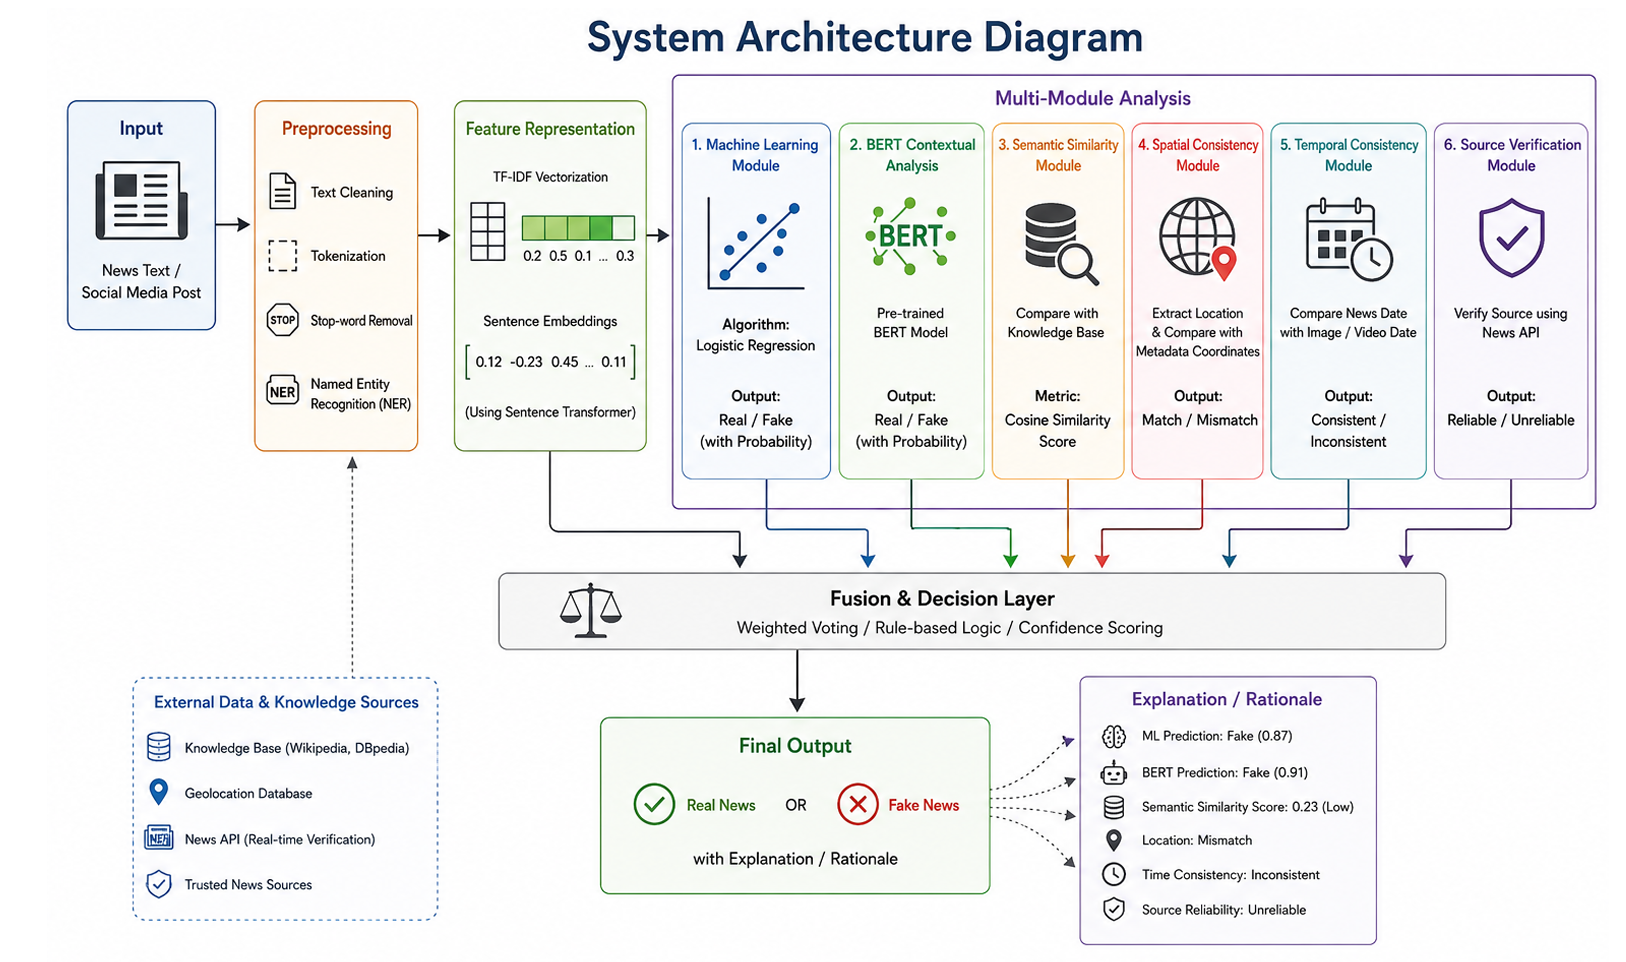
\includegraphics[width=\linewidth]{system_architecture.png}
\caption{System Architecture of the Proposed Hybrid Fake News Detection System.}
\label{fig:arch}
\end{figure}

\begin{figure}[htbp]
\centering
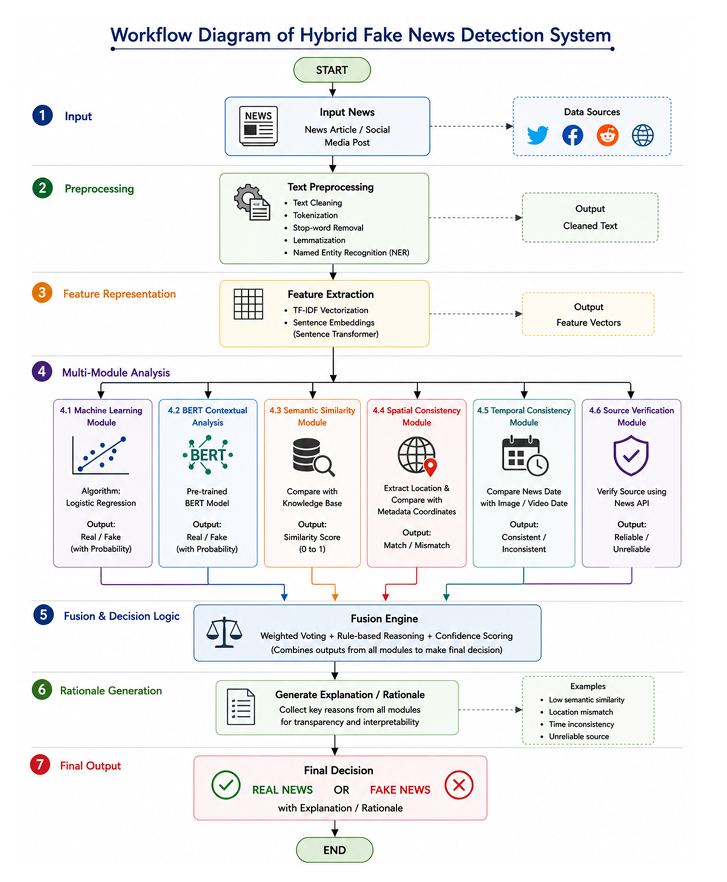
\includegraphics[width=\linewidth]{workflow_diagram.png}
\caption{Workflow Diagram of the Proposed System.}
\label{fig:workflow}
\end{figure}

\section{Results and Discussion}
The proposed Hybrid Neuro-Symbolic Fake News Detection System was evaluated using benchmark datasets and custom forensic test cases. The TF-IDF + Logistic Regression baseline achieved good classification performance, while the BERT model improved contextual understanding and reduced semantic ambiguity.

\begin{figure}[htbp]
\centering
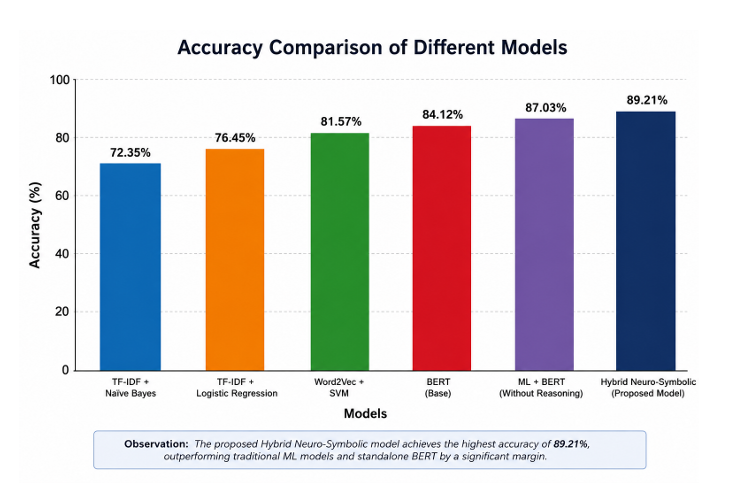
\includegraphics[width=\linewidth]{accuracy_chart.png}
\caption{Accuracy Comparison of Different Models.}
\label{fig:accuracy}
\end{figure}

\begin{table}[htbp]
\caption{Performance Comparison Across Models}
\label{tab:performance}
\centering
\begin{tabular}{lc}
\toprule
\textbf{Model Architecture} & \textbf{Accuracy (\%)} \\
\midrule
TF-IDF + Naive Bayes & 72.35\% \\
TF-IDF + Logistic Regression & 76.45\% \\
Word2Vec + SVM & 81.57\% \\
BERT (Base) & 84.12\% \\
ML + BERT (Without Reasoning) & 87.03\% \\
\textbf{Hybrid Neuro-Symbolic (Proposed)} & \textbf{89.21\%} \\
\bottomrule
\end{tabular}
\end{table}

\begin{figure}[htbp]
\centering
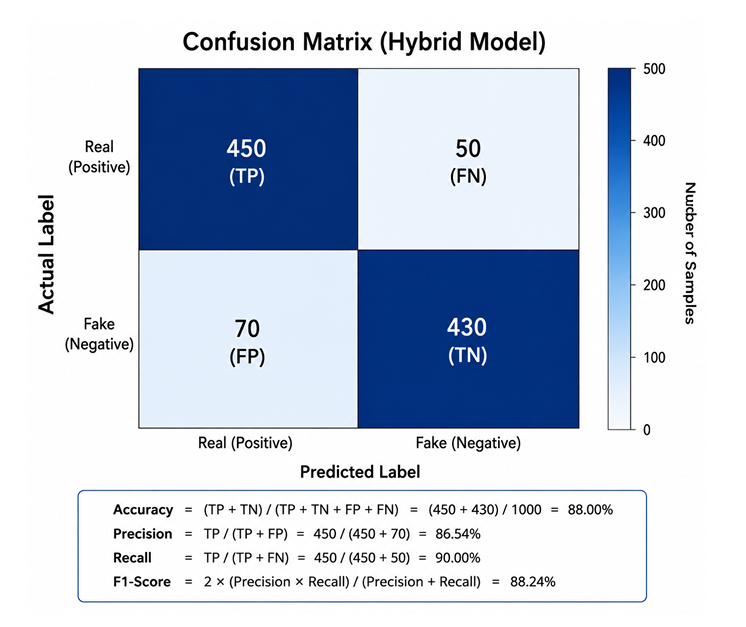
\includegraphics[width=\linewidth]{confusion_matrix.png}
\caption{Confusion Matrix of the Hybrid Model.}
\label{fig:cm}
\end{figure}

The forensic verification module effectively identified spatial mismatches, recycled media, and unsupported claims. Semantic similarity analysis improved factual grounding by comparing input claims with trusted knowledge base statements.

Based on a test cohort of 1000 samples (450 True Positives, 430 True Negatives, 70 False Positives, 50 False Negatives):
\begin{align}
\text{Accuracy} &= \frac{TP + TN}{TP + TN + FP + FN} = \frac{450 + 430}{1000} = 88.00\% \\
\text{Precision} &= \frac{TP}{TP + FP} = \frac{450}{450 + 70} = 86.54\% \\
\text{Recall} &= \frac{TP}{TP + FN} = \frac{450}{450 + 50} = 90.00\% \\
\text{F1-Score} &= 2 \times \frac{\text{Precision} \times \text{Recall}}{\text{Precision} + \text{Recall}} = 88.24\%
\end{align}

\begin{figure}[htbp]
\centering
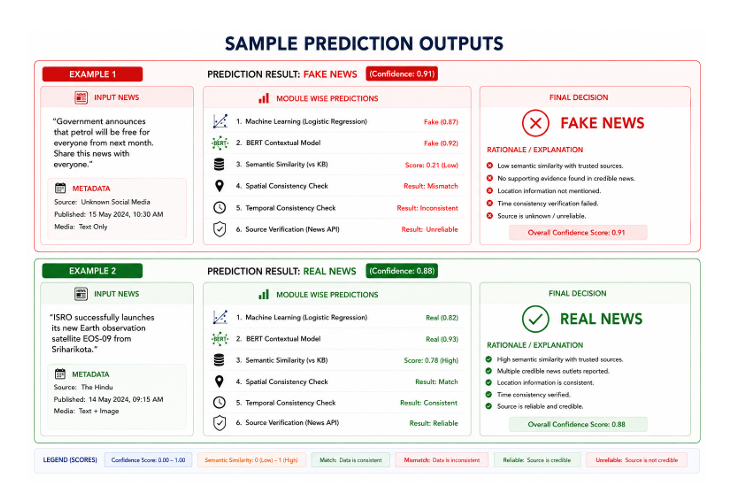
\includegraphics[width=\linewidth]{sample_outputs.png}
\caption{Sample Fake News Prediction Outputs with Explanations.}
\label{fig:samples}
\end{figure}

The rationale generation module enhanced explainability by providing structured reasoning factors such as low semantic similarity, location mismatch, temporal inconsistency, and unreliable source detection alongside the prediction confidence.

\section{Conclusion}
This project presented a Hybrid Neuro-Symbolic Fake News Detection System combining Machine Learning, BERT-based Deep Learning, semantic similarity verification, forensic analysis, and explainable reasoning. Unlike traditional black-box classifiers, the proposed system provides rationale explanations along with predictions, improving transparency and trustworthiness.

The integration of semantic verification, temporal consistency analysis, spatial consistency verification, and source validation improved the robustness of the system against misleading content. Experimental evaluation demonstrated an accuracy of approximately 89\%, validating the effectiveness of the hybrid approach. Future work includes real-time multimodal verification, deepfake video analysis, and scalable web deployment.

\begin{thebibliography}{00}
\bibitem{shu2017fake} K. Shu, A. Sliva, S. Wang, J. Tang, and H. Liu, ``Fake News Detection on Social Media: A Data Mining Perspective,'' \textit{ACM SIGKDD Explorations Newsletter}, vol. 19, no. 1, pp. 22--36, 2017.
\bibitem{devlin2019bert} J. Devlin, M. Chang, K. Lee, and K. Toutanova, ``BERT: Pre-training of Deep Bidirectional Transformers for Language Understanding,'' in \textit{Proc. NAACL-HLT}, 2019, pp. 4171--4186.
\bibitem{vaswani2017attention} A. Vaswani et al., ``Attention Is All You Need,'' in \textit{Proc. Adv. Neural Inf. Process. Syst. (NIPS)}, 2017, pp. 5998--6008.
\bibitem{ahmed2017detecting} H. Ahmed, I. Traore, and S. Saad, ``Detecting Opinion Spams and Fake News Using Text Classification,'' \textit{Security and Privacy}, vol. 1, no. 1, 2018.
\bibitem{mikolov2013efficient} T. Mikolov, K. Chen, G. Corrado, and J. Dean, ``Efficient Estimation of Word Representations in Vector Space,'' in \textit{Proc. Int. Conf. Learn. Represent. (ICLR)}, 2013.
\bibitem{pennington2014glove} J. Pennington, R. Socher, and C. D. Manning, ``GloVe: Global Vectors for Word Representation,'' in \textit{Proc. EMNLP}, 2014, pp. 1532--1543.
\bibitem{ribeiro2016why} M. T. Ribeiro, S. Singh, and C. Guestrin, ``"Why Should I Trust You?": Explaining the Predictions of Any Classifier,'' in \textit{Proc. ACM SIGKDD Int. Conf. Knowl. Discov. Data Min. (KDD)}, 2016, pp. 1135--1144.
\bibitem{goodfellow2016deep} I. Goodfellow, Y. Bengio, and A. Courville, \textit{Deep Learning}. MIT Press, 2016.
\bibitem{shu2019beyond} K. Shu et al., ``Beyond News Contents: The Role of Social Context for Fake News Detection,'' in \textit{Proc. WSDM}, 2019, pp. 312--320.
\bibitem{jurafsky2023speech} D. Jurafsky and J. H. Martin, \textit{Speech and Language Processing}, 3rd ed. Pearson Education, 2023.
\end{thebibliography}

\end{document}